\section{Trial Wave Function}
An accurate trial wave function can drastically improve the accuracy of a variational QMC method such as VMC. Most highly accurate trial wave functions are entirely computationally intractable and are never implemented in QMC methods. In addition to being accurate and computationally tractable we need wave functions that satisfy known physical properties such as cluster decomposition as well as having an overall antisymmetry with respect to particle exchange due to nucleons obeying fermi statistics.

Cluster decomposition arises from the physical intuition that the wave function of two separate, non-interacting systems, $A$ and $B$ as in Figure~\ref{fig:cluster}, can be written as the product of their respective wave functions.
\begin{figure}[h]
   \centering
   \begin{tikzpicture}[>=latex,scale=0.5]
      \shade[ball color=blue!10!] (-4.0,0.85) circle (1) ;
      \shade[ball color=blue!10!] (-2.5,-0.85) circle (1) ;
      \shade[ball color=blue!10!] (4.0,1.35) circle (1) ;
      \shade[ball color=blue!10!] (2.5,0.00) circle (1) ;
      \draw (-3.5,-2.5) node{\large $\ket{A}$};
      \draw (3.5,-1.5) node{\large $\ket{B}$};
   \end{tikzpicture}
   \caption{Two non interacting systems $A$ and $B$, whose composite wave function is the product $\ket{A+B}=\ket{A}\ket{B}$.}
   \label{fig:cluster}
\end{figure}
Mathematically this can be represented as a product of $n$-body functions, where $n$ is often 1 or 2 in our situation, though it could be higher. If a system is not cluster decomposable then unphysical correlations between non-interacting systems can occur.

The second property is that the wave function be antisymmetric overall. Since nucleons are fermions and the only degrees of freedom used in these calculations the product of different pieces of the wave function must be antisymmetric. Recent work in QMC has successfully included bosonic degrees of freedom such as pions \cite{madeira2018}, however that is not the case in this work.

%\begin{figure}[h!]
%   \centering
%   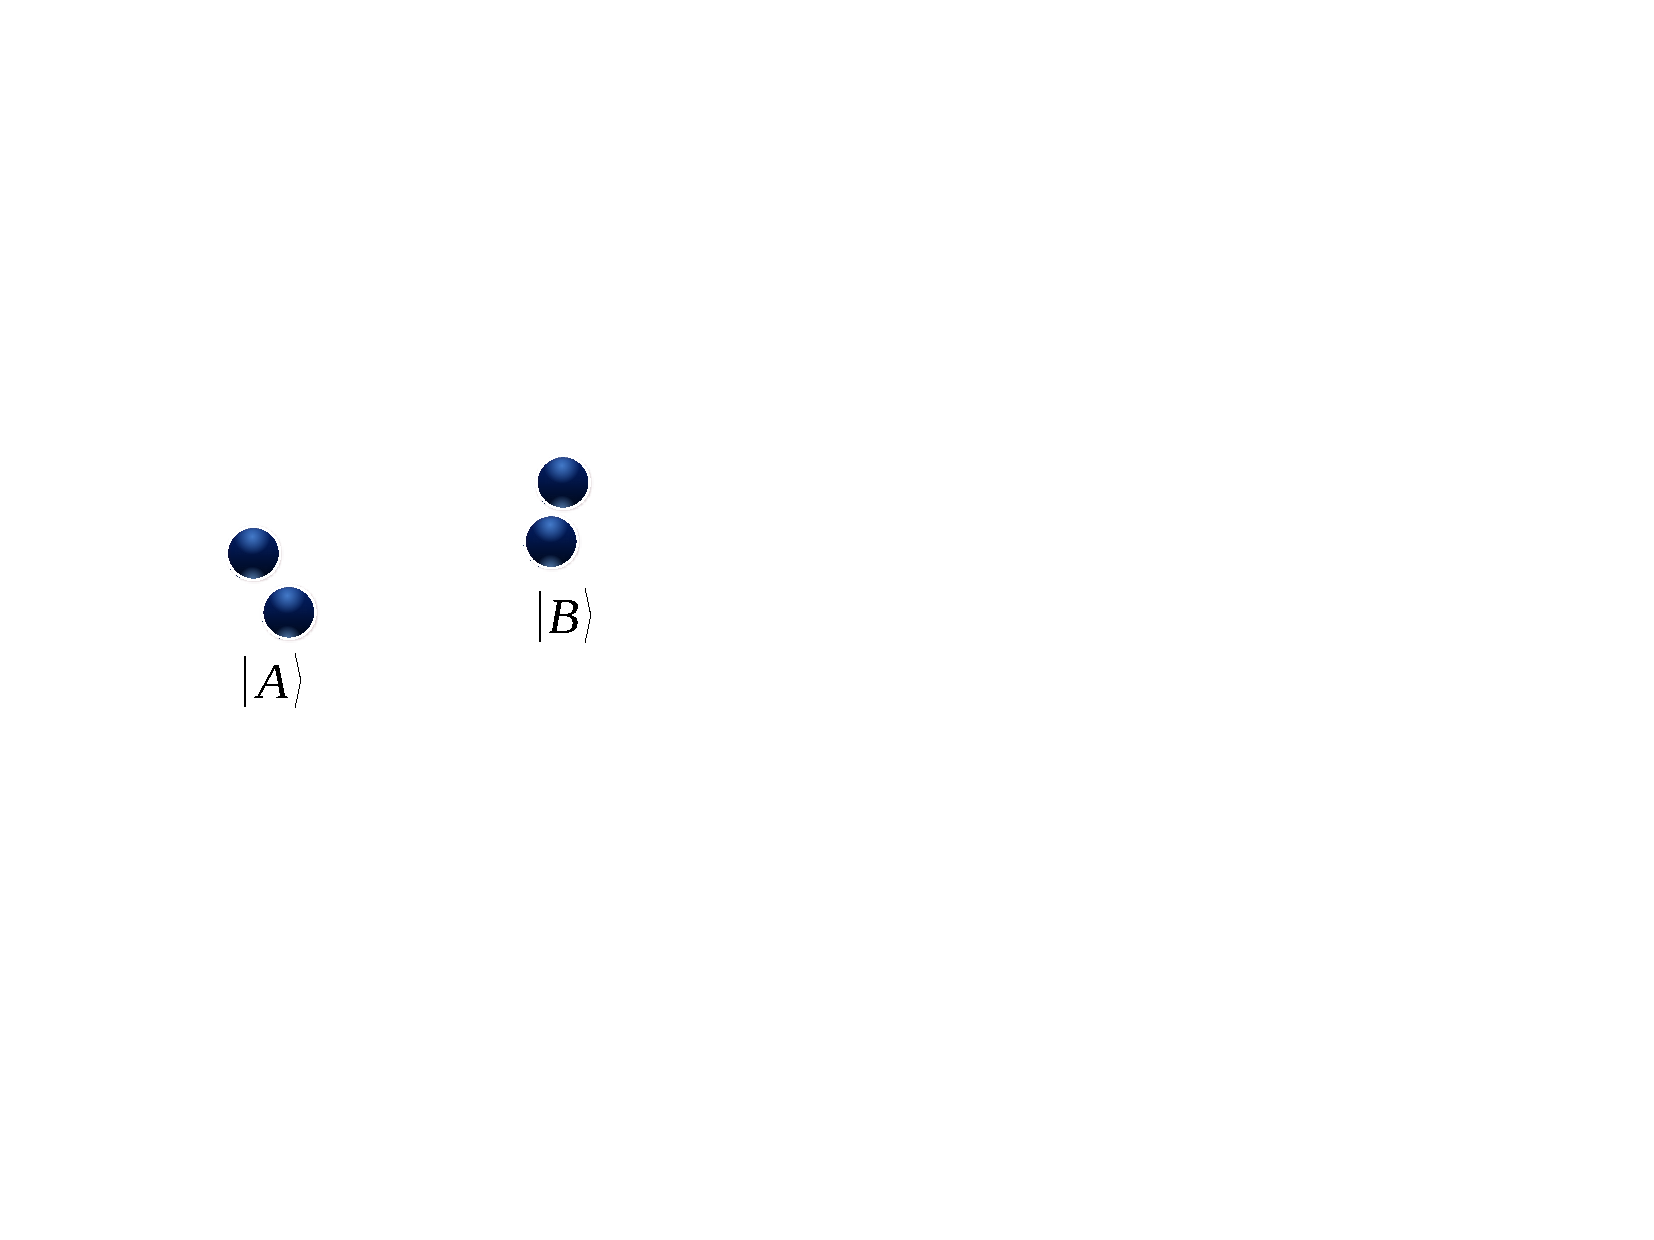
\includegraphics[width=\textwidth]{figures/cluster.pdf}
%   \caption{Energy per nucleon for ${}^4$He and ${}^{16}$O as calculated with linear, independent pair and quadratic correlations. Also, the energy per nucleon of symmetric nuclear matter of 28 particles in a periodic box with density $\rho=0.16$fm$^{-3}$. All calculations are compared to their expected values.}
%   \label{fig:cluster}
%\end{figure}

\subsection{Slater Determinant}
One of the simplest wave functions that satisfies the two properties specified above is the Slater determinant. The Slater determinant has been the starting place for a variety of many-body calculations in nuclear and condensed matter physics alike. In condensed matter the many-body wave functions will often be written in terms of a sum of weighted Slater determinants, where some methods have been able to use a sum of up to 2 billion determinants \cite{huron1973,li2018}. In nuclear physics a single determinant is often used for closed shell calculations and a sum of a small number, $\mathcal{O}(10)$, of weighted determinants is used for open shell systems. A Slater determinant is an antisymmetrized product of single particle (non-interacting) wave functions
\begin{equation}
   \Psi_{SD}(\R,S) = \mathcal{A} \left[\phi_1(\r_1)\phi_2(\r_2) \ldots \phi_A(\r_A)\right] =
   \begin{vmatrix}
      \phi_1(\r_1) & \phi_1(\r_2) & \ldots & \phi_1(\r_A) \\
      \phi_2(\r_1) & \phi_2(\r_2) & \ldots & \phi_2(\r_A) \\
      \vdots & \vdots & \ddots & \vdots \\
      \phi_K(\r_1) & \phi_K(\r_2) & \ldots & \phi_K(\r_A) \\
   \end{vmatrix},
\end{equation}
where $\R$ and $S$ are the spatial and spin coordinates of the walkers, $\mathcal{A}$ is the antisymitrization operator, and the $\phi_i(\r_j)$ are the overlap of the walker positions with the model single particle states. The single particle model states are made up of a radial and spin, iso-spin dependent parts,
\begin{equation}
   \phi_k = \Phi_{nj}\left[C_{c_l,m_s}^j Y_{l,m_l}(\hat{r}_i)\chi_s(s_i)\right]_{j,m_j},
\end{equation}
where $\Phi_{nj}$ is the radial part and the rest contains the spherical harmonics $Y_{l,m_l}(\hat{r}_I)$ and spin and iso-spin states where the Clebsch-Gordan coefficients ensure the correct $j$ and $m_j$ quantum numbers, and the different states are given by the index $k$. To accurately describe the wave function of an open shell nuclei each state with the correct total angular momentum and parity $J^\pi$ and isospin $T$ is included as a seperate Slater determinant.
\begin{equation}
   \braket{\R S}{\Phi}_{J^\pi,T} = \sum\limits_n c_n D\{\phi_k(\r_i,s_i)\}
\end{equation}
Here the $c_n$ coefficients are variational parameters used to minimize the energy given a set of possible state configurations. One of the simplest examples of an open shell nuclei would be $^6$He whose ground state is a $J^\pi = 0^+$ state. The two protons and two of the neutrons could be in the full $(1S_{1/2})^2$ shell while the two remaining neutrons could be in the $(1P_{3/2})^2$ shell with their $m_j=\pm 3/2, \pm 1/2$ values being equal and opposite to ensure that $J=0$. This state has two possible determinants. Other possible configurations for the two remaining neutrons would be $(1P_{1/2})^2$ with one possible determinant, $(1D_{5/2})^2$ with three possible determinants, $(2S_{1/2})^2$ with one possible determinant and $(1D_{3/2})^2$ with two possible determinants giving a total of nine possible determinants. Notice that the two neutrons could be in a combination of $S$ and $D$ shells but never an $S$ and $P$ or $D$ and $P$ to ensure the parity of the state is positive. The number of determinants used for open shell nuclei will control how accurate the trial wave function is but for closed shell nuclei such as $^4$He or $^{16}$O a single slater determinant describing the full shell configuration is sufficient.

The radial part $\Phi_{nj}$ of the single particle states are obtained as bound state solutions to the single particle Schr\"odinger equation with a Woods-Saxon potential wine-bottle potential.
\begin{equation}
   v(r) = V_s\left[\frac{1}{1+e^{(r-r_s)/a_s}} + \alpha_se^{(-r/\rho_s)^2}\right]
\end{equation}
Here the parameters, $V_s, r_s, a_s, \alpha_s$ and $\rho_s$ are variational parameters used to shape the potential to obtain a minimum in energy.

%As an illustrative example consider the deuteron. The deuteron is in a iso-spin singlet state, $\frac{1}{\sqrt{2\pi}}(\ket{pn}-\ket{np})$. To show how the model state, $\ket{\Phi}$ would be built for this I will assume all entries are 1, though in practice the could all take on different numbers to account for the different spacial and spin dependencies of the state. Let's assume that both the neutron and the proton are in a spin up state. In this case the $\Phi(k,i)$ terms, where $k,i=1,2$, would take on the following values.
%\begin{align}
%   \phi(1,1)&=(1,0,0,0)=p\uparrow_1 \\
%   \phi(2,1)&=(0,0,1,0)=n\uparrow_1 \\
%   \phi(1,2)&=(1,0,0,0)=p\uparrow_2 \\
%   \phi(2,2)&=(0,0,1,0)=n\uparrow_2
%\end{align}
%The determinant of the Slater matrix can then be written as
%\begin{equation}
%\Psi_T=\det(S)=
%\begin{vmatrix}
%    \braket{k_1}{s_1} & \braket{k_1}{s_2} \\
%    \braket{k_2}{s_1} & \braket{k_2}{s_2}
%\end{vmatrix}
%=
%\begin{vmatrix}
%    p_1 & p_2 \\
%    n_1 & n_2
%\end{vmatrix}
%=
%p_1n_2-n_1p_2,
%\end{equation}
%which is the singlet state that we wanted to start with.

The Slater determinant is a mean-field wave function and is often used with Jastrow type short range correlations.
\begin{equation}
   \braket{\R S}{\psi_T} = \bra{\R S}\prod\limits_{i<j}f(r_{ij}) \ket{\phi}_{SD}
   \label{equ:jastrow}
\end{equation}
These correlations are spin-isospin independent and depend only on the particle separation and improve upon the uncorrelated Slater determinant wave function significantly. To maintain the cluster decomposition the functions $f(r_{ij})$ must go to unity for large particle seperations. In this work we have used Slater determinant wave functions with a Jastrow factor and spin-isospin dependent correlations which will be discussed in a later section. \red{ADD PLOT AND CITATION BACKING THIS CLAIM HERE}.

\subsection{Pfaffian Wave Function}
\red{Explain why it would be nice to have a pfaffian instead of a determinant and maybe mention some of the results related to superfluidity etc. \\}
Another wave function that obeys these properties is the paired Pfaffian wave function. This wave function was developed to describe Cooper pairs which form when, at low temperature, paired fermions, such as electrons or liquid $^3$He, are energetically favorable to free particles \cite{cooper1956,leggett1975}. This idea was then expanded and used to explain superconductivity as the condensation of these bosonic cooper pairs into the ground state \cite{bardeen1957,bardeen1957_2}. A Pfaffian wave function was then introduced to describe these paired systems by Bouchaud {\it et al.} in 1988 \cite{bouchaud1988}.

The BCS, or Pfaffian, pairing wave function can be written as an antisymmetrized product of pairing wave functions, thus keeping the antisymmetry of the constituent fermions explicitly. That is,
\begin{equation}
   \Psi_{BCS}(\R S) = \mathcal{A}\left[\phi(\r_1,s_1,\r_2,s_2)\phi(\r_3,s_3,\r_4,s_4)\ldots\phi(\r_{A-1},s_{A-1},\r_A,s_A)\right],
\end{equation}
where $\mathcal{A}$ is the antisymmetrization operator, $\r_i$ and $s_i$ are the walkers positions and spins, and $\phi$ are the pairing functions which can be separated into a spatial part, whose form is determined by the system, and a spin-isospin part, which are often written in terms of singlet and triplet states.

This wave function, like the Slater determinant, can be used with additional Jastrow-like correlations as in equation~\ref{equ:jastrow}.
\begin{equation}
   \braket{\R S}{\psi_T} = \bra{\R S}\prod\limits_{i<j}f(r_{ij}) \ket{\phi}_{BCS}
\end{equation}
For more information and a more detailed use and description of this wave function we refer the reader to \cite{madeira2018_diss}.

\subsection{Spin-Isospin Dependent Correlations}
\red{Explain what properties you need, etc.}
The nuclear Hamiltonian has a strong spin-isospin dependent part and to ensure good overlap with the trial wave function, the wave function must include spin-isospin dependent correlations. From here on I will be using the Slater determinant for the long-range part of the wave function. To improve on the Jastrow correlations in equation~\ref{equ:jastrow}, spin-isospin dependent correlations can be included that obey the properties of cluster decomposability and overall antisymmetry.

We have come up with two such correlations, the exponentially correlated,
\begin{equation}
   \Psi_{\text{exp}}(\R, S) = \bra{\R S}\left[\prod\limits_{i<j}f_c(r_{ij})\right] e^{\sum\limits_{i<j}\sum\limits_{p}f_p(r_{ij})\Opij}\ket{\phi}
   \label{equ:exppsi}
\end{equation}
and the symmetrized product wave functions,
\begin{equation}
   \Psi_{\text{SP}}(\R, S) = \bra{\R S}\left[\prod\limits_{i<j}f_c(r_{ij})\right] \left[\mathcal{S}\prod\limits_{i<j}\left(1+\sum\limits_p\fpij\Opij\right)\right] \ket{\phi}.
   \label{equ:prodpsi}
\end{equation}
where the $S$ is the symmetrization operator, the $f_c(r_{ij}$ are the same Jastrow correlations as before, and the $\Opij$ are the operators from the AV6' potential, $(1,\si\cdot\sj,S_{ij})\otimes(1,\ti\cdot\tj)$, where the tensor term is $S_{ij} = 3\si\cdot\hat{r}_{ij}\sj\cdot\hat{r}_{ij}-\si\cdot\sj$. The $f_p(r_{ij})$ functions contain variational parameters and the functional form is determined by solving a Schr\"odinger-type equation with the constraint that the wave function be continuous at the healing distance \cite{pandharipande1979,pandharipande1977}.

The exponentially correlated wave function obeys cluster decomposition as long as the correlating functions, $f_p(r_{ij})$ go to zero as the particle seperation increases. This dampens out unphysical long-range particle correlations between physically separated systems. Also, due to the sum over particle pairs in the exponential, no explicit symmetrization is needed.

The symmetrized product wave function, introduced by Pandharipande and Wiringa in 1979 \cite{pandharipande1979}, requires an explicit symmetrization and is not obviously cluster decomposable. The addition of the 1 is need to ensure cluster decomposability because these $f_p(r_{ij}$ functions also approach zero as particle seperation increases.

When expanded to linear order these correlations are identical and can be written as
\begin{equation}
   \ket{\psi_T}_\text{lin} = \left[\prod\limits_{i<j}f_c(r_{ij})\right] \left(1+\sum\limits_{i<j}\sum\limits_p\fpij\Opij\right) \ket{\phi}.
\end{equation}
These correlations are symmetric, allowing for the full wave function to be antisymmetric, however it has lost the cluster decomposability in the approximation. This is because the pair correlations are summed instead of beign inside a product. For higher orders expansions these two wave functions differ by commutation relations as well as the inclusion of additional correlation pairs. Until recently, only correlations up to linear order in the expansion were used for AFDMC calculations. Calculations for GFMC use a much better wave function, but have been limited to small nuclei up to $^{12}$C. Calculations done with the AFDMC method have been slowely improving the trial wave function used, as a better wave function is surely needed to describe larger systems. In 2007 AFDMC binding energy calculations were done for $^4$He, $^{16}$O, and $^{40}$Ca using only the Jastrow correlations \cite{gandolfi2007}. These calculations were repeated in 2014 but with the addition of linear correlations \cite{gandolfi2014} and I have plotted the respective results compared to current experimental values here for comparison.
\begin{figure}[h!]
   \centering
   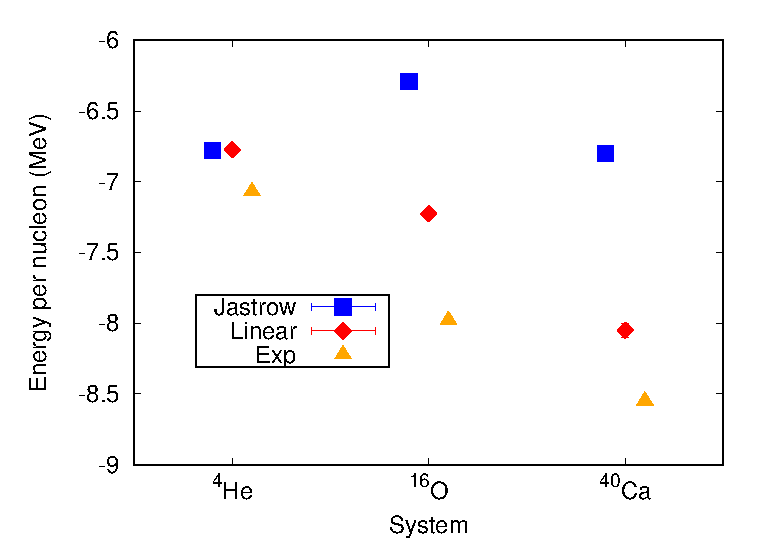
\includegraphics[width=0.7\textwidth]{figures/energy_jaslin.eps}
   \caption{Binding energy calculations done with Jastrow correlations \cite{gandolfi2007} compared to Jastrow plus linear spin-isospin dependent correlations \cite{gandolfi2014} all compared to experimental results. All calculations were done with AFDMC and the AV6$'$ potential.}
   \label{fig:energy_jaslin}
\end{figure}
In figure~\ref{fig:energy_jaslin} it is clear to see that the additional spin-isospin correlations are important for both systems larger than $^4$He.

\subsubsection{Quadratic Correlations}
In this project we have included correlations up to quadratic order which includes up to 4 nucleons begin correlated at once. When expanded to quadratic order the symmetrized product wave function, equation~\ref{equ:prodpsi}, becomes
\begin{equation}
   \begin{split}
      \ket{\psi_T}_\text{quad} = \Bigg[\prod\limits_{i<j}&f_c(r_{ij})\Bigg] \Bigg[1+\fOpij \\
         & + \frac{1}{2}\fOpij\fOqklquad \Bigg] \ket{\phi}.
   \end{split}
   \label{equ:fullquadcorr}
\end{equation}
The subscripts on the sums which describe which correlations are allowed can be hard to visualize and so these correlation diagrams are used.
\begin{figure}[h]
\newcommand\shift{2.0}
\newcommand\vshift{-1.5} %vertical shift
\newcommand\tshift{0.05} %tiny shift
\newcommand\sep{0.75}
   \centering
   \begin{tikzpicture}[>=latex,scale=1.0]
      \draw (-2*\sep,\sep/2.0) node{\large Allowed};
      \draw (-2*\sep,\sep/2.0+\vshift) node{\large Not Allowed};

      \filldraw[black] (0*\shift,0)          circle (2pt) node[anchor=east] {\large j};
      \filldraw[black] (0*\shift,\sep)       circle (2pt) node[anchor=east] {\large i};
      \filldraw[black] (0*\shift+\sep,0)     circle (2pt) node[anchor=west] {\large l};
      \filldraw[black] (0*\shift+\sep,\sep)  circle (2pt) node[anchor=west] {\large k};
      \draw[black, ultra thick] (0*\shift,\sep) -- (0*\shift,0); %i-j
      \draw[black, ultra thick] (0*\shift+\sep,\sep) -- (0*\shift+\sep, 0); %k-l

      \filldraw[black] (1*\shift,0)          circle (2pt) node[anchor=east] {\large k};
      \filldraw[black] (1*\shift,\sep)       circle (2pt) node[anchor=east] {\large i};
      \filldraw[black] (1*\shift+\sep,0)     circle (2pt) node[anchor=west] {\large l};
      \filldraw[black] (1*\shift+\sep,\sep)  circle (2pt) node[anchor=west] {\large j};
      \draw[black, ultra thick] (1*\shift,\sep) -- (1*\shift+\sep,\sep); %i-j
      \draw[black, ultra thick] (1*\shift,0) -- (1*\shift+\sep,0); %k-l

      \filldraw[black] (2*\shift,0)          circle (2pt) node[anchor=east] {\large l};
      \filldraw[black] (2*\shift,\sep)       circle (2pt) node[anchor=east] {\large i};
      \filldraw[black] (2*\shift+\sep,0)     circle (2pt) node[anchor=west] {\large j};
      \filldraw[black] (2*\shift+\sep,\sep)  circle (2pt) node[anchor=west] {\large k};
      \draw[black, ultra thick] (2*\shift,\sep) -- (2*\shift+\sep,0); %i-j
      \draw[black, ultra thick] (2*\shift+\sep,\sep) -- (2*\shift,0); %k-l

      \filldraw[black] (3*\shift,0)          circle (2pt) node[anchor=east] {\large j};
      \filldraw[black] (3*\shift,\sep)       circle (2pt) node[anchor=east] {\large i,k};
      \filldraw[black] (3*\shift+\sep,0)     circle (2pt) node[anchor=west] {\large };
      \filldraw[black] (3*\shift+\sep,\sep)  circle (2pt) node[anchor=west] {\large l};
      \draw[black, ultra thick] (3*\shift,\sep) -- (3*\shift,0); %i-j
      \draw[black, ultra thick] (3*\shift,\sep) -- (3*\shift+\sep,\sep); %k-l

      \filldraw[black] (4*\shift,0)          circle (2pt) node[anchor=east] {\large k};
      \filldraw[black] (4*\shift,\sep)       circle (2pt) node[anchor=east] {\large i};
      \filldraw[black] (4*\shift+\sep,0)     circle (2pt) node[anchor=west] {\large j,l};
      \filldraw[black] (4*\shift+\sep,\sep)  circle (2pt) node[anchor=west] {\large };
      \draw[black, ultra thick] (4*\shift,\sep) -- (4*\shift+\sep,0); %i-j
      \draw[black, ultra thick] (4*\shift,0) -- (4*\shift+\sep,0); %k-l

      \filldraw[black] (2*\shift,\vshift)             circle (2pt) node[anchor=east] {\large j,l};
      \filldraw[black] (2*\shift,\sep+\vshift)        circle (2pt) node[anchor=east] {\large i,k};
      \filldraw[black] (2*\shift+\sep,\vshift)        circle (2pt) node[anchor=west] {\large };
      \filldraw[black] (2*\shift+\sep,\sep+\vshift)   circle (2pt) node[anchor=west] {\large };
      \draw[black, ultra thick] (2*\shift-\tshift,\sep+\vshift) -- (2*\shift-\tshift,\vshift); %i-j
      \draw[black, ultra thick] (2*\shift+\tshift,\sep+\vshift) -- (2*\shift+\tshift,\vshift); %k-l
   \end{tikzpicture}
   \caption{Diagrams used to visualize which correlations are included in the quadratic correlations in equation~\ref{equ:fullquadcorr}.}
   \label{fig:quaddiagrams}
\end{figure}
All pair correlations are included in this wave function except pairs that are directly correlated with themselves, e.g. $\mathcal{O}_{23}\mathcal{O}_{23}$, where $\mathcal{O}_{ij}$ is a product of single particle operators such as $\si\cdot\sj$ and $\mathcal{O}_{ij}=\mathcal{O}_{ji}$ due to the operators on different particles operating in different Hilbert spaces. For correlations where the same particle is included twice, the correlation operators do not commute and that term must be explicitly symmetrized. Currently in equation~\ref{equ:fullquadcorr} and in the code all quadratic terms are symmetrized, e.g. the correlation $\mathcal{O}_{12}\mathcal{O}_{34}$ is symmetrized as $\frac{1}{2}\left(\mathcal{O}_{12}\mathcal{O}_{34}+\mathcal{O}_{34}\mathcal{O}_{12}\right)$ even though only terms like $\mathcal{O}_{12}\mathcal{O}_{13}$ need this explicit symmetrization. This adds needless calculation time, but as I'll show, these terms don't seem to be important at all and can be omitted completely.

If the exponentially correlated wave function, equation~\ref{equ:exppsi}, is expanded in the typical way, i.e. $\exp(A) = 1 + A + \frac{1}{2}A^2 \ldots$, then the quadratic correlations for the exponential wave function become
\begin{equation}
   \begin{split}
      \ket{\psi_T}_\text{exp\_quad} = \Bigg[\prod\limits_{i<j}&f_c(r_{ij})\Bigg] \Bigg[1+\fOpij \\
         & + \frac{1}{2}\fOpij\fOqklexpquad \Bigg] \ket{\phi}.
   \end{split}
   \label{equ:expquadcorr}
\end{equation}
Unlike the quadratic correlations derived from the symmetrized product this wave function includes all of the the terms in figure~\ref{fig:quaddiagrams}. There is not a large difference between these wave functions up to quadratic order and for here forward all references to quadratic correlations will refer to the expansion from the symmetrized product wave function.

Another way to include quadratic correlations is to only include terms that do not correlate the same particle twice leaving only independent pair correlations. This is the same whether you start from the exponentially correlated or the symmetrized product wave function and it can be written as
\begin{equation}
   \begin{split}
      \ket{\psi_T}_\text{ip} = \Bigg[\prod\limits_{i<j}&f_c(r_{ij})\Bigg] \Bigg[1+\fOpij \\
      & + \fOpij\fOqklip \Bigg] \ket{\phi}
   \end{split}
   \label{equ:ipquadcorr}
\end{equation}
and the independent pair sum can be visualized as in figure~\ref{fig:ipdiagrams}.
\begin{figure}[h]
\newcommand\shift{2.2}
\newcommand\vshift{-1.5} %vertical shift
\newcommand\tshift{0.05} %tiny shift
\newcommand\sep{0.75}
   \centering
   \begin{tikzpicture}[>=latex,scale=1.0]
      \draw (-3*\sep,\sep/2.0) node{\large Allowed};
      \draw (-3*\sep,\sep/2.0+\vshift) node{\large Not Allowed};

      \filldraw[black] (0*\shift,0)          circle (2pt) node[anchor=east] {\large j};
      \filldraw[black] (0*\shift,\sep)       circle (2pt) node[anchor=east] {\large i};
      \filldraw[black] (0*\shift+\sep,0)     circle (2pt) node[anchor=west] {\large l};
      \filldraw[black] (0*\shift+\sep,\sep)  circle (2pt) node[anchor=west] {\large k};
      \draw[black, ultra thick] (0*\shift,\sep) -- (0*\shift,0); %i-j
      \draw[black, ultra thick] (0*\shift+\sep,\sep) -- (0*\shift+\sep, 0); %k-l

      \filldraw[black] (1*\shift,0)          circle (2pt) node[anchor=east] {\large k};
      \filldraw[black] (1*\shift,\sep)       circle (2pt) node[anchor=east] {\large i};
      \filldraw[black] (1*\shift+\sep,0)     circle (2pt) node[anchor=west] {\large l};
      \filldraw[black] (1*\shift+\sep,\sep)  circle (2pt) node[anchor=west] {\large j};
      \draw[black, ultra thick] (1*\shift,\sep) -- (1*\shift+\sep,\sep); %i-j
      \draw[black, ultra thick] (1*\shift,0) -- (1*\shift+\sep,0); %k-l

      \filldraw[black] (2*\shift,0)          circle (2pt) node[anchor=east] {\large l};
      \filldraw[black] (2*\shift,\sep)       circle (2pt) node[anchor=east] {\large i};
      \filldraw[black] (2*\shift+\sep,0)     circle (2pt) node[anchor=west] {\large j};
      \filldraw[black] (2*\shift+\sep,\sep)  circle (2pt) node[anchor=west] {\large k};
      \draw[black, ultra thick] (2*\shift,\sep) -- (2*\shift+\sep,0); %i-j
      \draw[black, ultra thick] (2*\shift+\sep,\sep) -- (2*\shift,0); %k-l

      \filldraw[black] (0*\shift,\vshift)          circle (2pt) node[anchor=east] {\large j};
      \filldraw[black] (0*\shift,\sep+\vshift)       circle (2pt) node[anchor=east] {\large i,k};
      \filldraw[black] (0*\shift+\sep,\vshift)     circle (2pt) node[anchor=west] {\large };
      \filldraw[black] (0*\shift+\sep,\sep+\vshift)  circle (2pt) node[anchor=west] {\large l};
      \draw[black, ultra thick] (0*\shift,\sep+\vshift) -- (0*\shift,\vshift); %i-j
      \draw[black, ultra thick] (0*\shift,\sep+\vshift) -- (0*\shift+\sep,\sep+\vshift); %k-l

      \filldraw[black] (1*\shift,\vshift)          circle (2pt) node[anchor=east] {\large k};
      \filldraw[black] (1*\shift,\sep+\vshift)       circle (2pt) node[anchor=east] {\large i};
      \filldraw[black] (1*\shift+\sep,\vshift)     circle (2pt) node[anchor=west] {\large j,l};
      \filldraw[black] (1*\shift+\sep,+\vshift)  circle (2pt) node[anchor=west] {\large };
      \draw[black, ultra thick] (1*\shift,\sep+\vshift) -- (1*\shift+\sep,\vshift); %i-j
      \draw[black, ultra thick] (1*\shift,\vshift) -- (1*\shift+\sep,\vshift); %k-l

      \filldraw[black] (2*\shift,\vshift)             circle (2pt) node[anchor=east] {\large j,l};
      \filldraw[black] (2*\shift,\sep+\vshift)        circle (2pt) node[anchor=east] {\large i,k};
      \filldraw[black] (2*\shift+\sep,\vshift)        circle (2pt) node[anchor=west] {\large };
      \filldraw[black] (2*\shift+\sep,\sep+\vshift)   circle (2pt) node[anchor=west] {\large };
      \draw[black, ultra thick] (2*\shift-\tshift,\sep+\vshift) -- (2*\shift-\tshift,\vshift); %i-j
      \draw[black, ultra thick] (2*\shift+\tshift,\sep+\vshift) -- (2*\shift+\tshift,\vshift); %k-l
   \end{tikzpicture}
   \caption{Diagrams used to visualize which correlations are included in the independent pair quadratic correlations in equation~\ref{equ:ipquadcorr}.}
   \label{fig:ipdiagrams}
\end{figure}
All terms where a particle is included twice in the correlation are ignored, as a results, all correlation operators commute and the correlations are explicitly symmetric. Neither of these of these correlations maintains cluster decomposability, however an effort to build an antisymmetric and cluster decomposable wave function from the exponentially correlated wave function will be discussed.

The energy and it's uncertainty are used to judge the convergence of a propagated wave function in QMC and so a good wave function needs to be able to reproduce known binding energies. To this end I have done binding energy calculations with the quadratic correlations derived from the symmetrized product for $^4$He, $^{16}$O, $^{40}$Ca, and symmetric nuclear matter (SNM) at saturation density, $\rho_0=0.16$ fm$^{-3}$, in a period box with 28 particles. The energy per particle for nuclei is plotted in figure~\ref{fig:energies} and the specific energies can be found in table~\ref{tab:energies}.
\begin{figure}[h!]
   \centering
   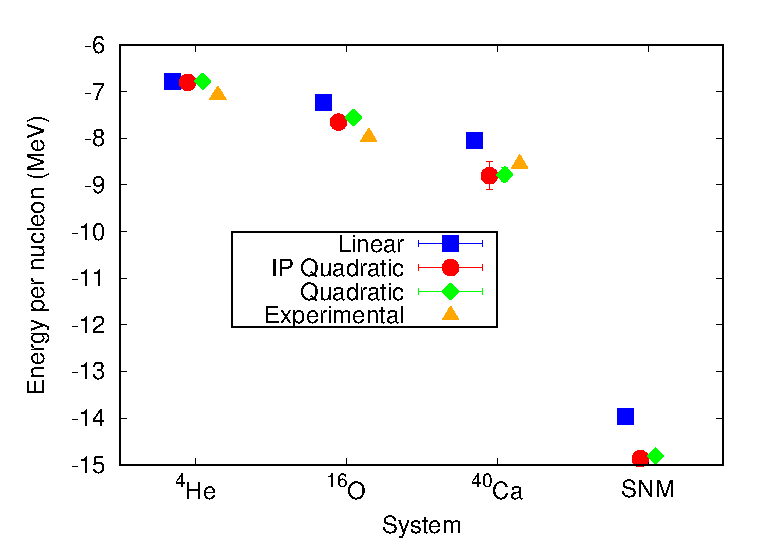
\includegraphics[width=0.7\textwidth]{figures/energy.eps}
   \caption{Energy per particle for small and medium closed shell nuclei with no Coulomb interaction with the AV6$'$ interaction. Each calculations was done with the linear, independent pair, and quadratic correlations. Energies are compared to experimental values where available and the statistical uncertainties are included.}
   \label{fig:energies}
\end{figure}
\begin{table}[htb]
   \centering
   \begin{tabular}{ccccc}
      \hline\hline
      System & Linear & Ind-Pair & Quadratic & Experimental \\
      \hline
      $^4${He}    & -6.785(10)   & -6.798(8) & -6.778(8)    & -7.074 \\   
      $^{16}${O}  & -7.23(6)     & -7.65(9)  & -7.55(8)     & -7.98  \\   
      $^{40}${Ca} & -8.05(8)     & -8.8(3)   & -8.78(15)    & -8.55  \\
      SNM         & -13.97(3)    & -14.87(4) & -14.70(11)   &        \\
      \hline\hline
   \end{tabular}
   \label{tab:energies}
   \caption{Energy per particle calculated with no Coulomb interaction with the AV6$'$ interaction. Each calculations was done with the linear, independent pair, and quadratic correlations. Energies are compared to experimental values where available and the statistical uncertainties are included. \blue{THEN PUT THE PLOT ABOVE THIS!}}
\end{table}
\red{Talk about the energy data and then make sure to include scaling and add a brief discussion about scaling (maybe even an estimate about how much the scaling ``would" be if quadratic correlations weren't fully symmetrized.}
\red{ALSO ADD THE PLOT FOR THE FIT TO SATURATION DONE WHEN TALKING TO ACHIM}
\red{\\After showing results make sure to state and all further calculations will be with the IP correlation, even if you say ``quadratic" correlations.}

\subsubsection{Exponential Correlations}
\red{Why aren't they working}

\subsubsection{Alessandro's correlations and $T^2$ fix to them - \red{Maybe just do $T^2$ fix and apply it to exponential correlations}}
